\documentclass[11pt,a4paper]{book}

\usepackage{latexsettings} % Verweis auf Datei latexsettings.sty
\usepackage{custom_commands}

% Titelseite
\title{Grundlagen der Fachdidaktik Physik}
\author{Axel Enders}
\date{\today}

\begin{document}

% Titelseite generieren
\begin{titlepage}
    \newgeometry{left=2.5cm, right=2.5cm, top=2.5cm, bottom=2.5cm} %andere Seitengeometrie fr Titelseite 5.8.24 J.Hlawatsch
	\vs{0.5cm}
	\begin{figure}[h]
	\centering
	
\includegraphics[scale=.1]{Logo_physikdidaktik_long.png}
	% \caption{Meine Grafik}
	\label{fig:Logo}
	\end{figure}
	
	\vs{1cm}
	\begin{center}
	\Large \textbf{Skript zur Vorlesung}
	\bip\bip
	\Huge \textbf{Grundlagen der \\ Fachdidaktik  Physik A}
	\bip\bip
	\Large
	(Stand WS 2024)
	\end{center}

	\vs{6cm}

	\begin{flushright}
		\textbf{Apl. Prof. Dr. Stefan Hilger} \\
			Mathematik, Didaktik der Mathematik  \\
			Katholische Universitaet Eichst\"att-Ingolstadt \\
			Ostenstrasse 26 - 28  \\
			85071 Eichst\"att \\
			Stefan.Hilger@ku.de \\

	\vs{0.5cm}

		\textbf{Prof. Dr. Axel Enders} \\
		Lehrstuhl f\"ur Experimentalphysik XI und Didaktik der Physik  \\
		Universit\"at Bayreuth  \\
		Universit\"atstrasse 30  \\
		95440 Bayreuth  \\
		axel.enders@uni-bayreuth.de
	\end{flushright}

\end{titlepage}

%---------------------------------------------------------------------------------------------------------------------------------
\newgeometry{left=2.5cm, right=2.5cm, top=2.5cm, bottom=2.5cm} %andere Seitengeometrie fr Vorwort und ToC 5.8.24 J.Hlawatsch
%---------------------------------------------------------------------------------------------------------------------------------
\newpage

\vs{3cm}
\section*{Vorwort}

Die urspr\"ungliche Version dieses Skriptes wurde von Apl. Prof. Dr. Stefan Hilger, Katholische Universit\"{a}t Eichst\"{a}tt-Ingolstadt, bis 2010 verfasst. Mit seiner freundlichen Genehmigung wird dieses Skript seit 2023 an der Universit\"{a}t Bayreuth als Begleitmaterial zur Physiklehrerbildung eingesetzt und am Lehrstuhl \emph{Experimentalphysik XI und Didaktik der Physik} kontinuierlich erweitert.   
\bip
\hs{10cm} Axel\ Enders


%---------------------------------------------------------------------------------------------------------------------------------
\newpage
\section*{Zur Nutzung dieses Skripts}

Dieses Skript wurde so formatiert, dass man beim Studium eigene Randnotizen an den Text anf\"{u}gen kann. Jeder Studierenden sei ermutigt, beim Lesen des Skripts eigene Randnotizen zu erstellen. Diese leider etwas aus der Mode gekommene Technik bietet beim Lernen erhebliche Vorteile:

\begin{itemize}
\item \textbf{F\"{o}rderung des aktiven Lesens:} Randnotizen ermutigen dazu, sich intensiv mit dem Text auseinanderzusetzen, um zentrale Punkte zu erkennen und hervorzuheben.

\item \textbf{Bessere Informationsverarbeitung:} Durch das Zusammenfassen von Informationen in eigenen Worten werden die Inhalte besser verstanden und im Ged\"{a}chtnis verankert.

\item \textbf{Erleichterung der sp\"{a}teren Wiederholung:} Randnotizen dienen als schnelle Erinnerungsst\"{u}tze und erleichtern das Wiederfinden wichtiger Informationen beim sp\"{a}teren Durchsehen des Textes.

\item \textbf{Unterst\"{u}tzung des kritischen Denkens:} Durch das Kommentieren des Gelesenen wird das kritische Denken gef\"{o}rdert, indem der Leser sich aktiv mit den Argumenten und Inhalten auseinandersetzt.

\item \textbf{Individuelle Strukturierung:} Randnotizen erm\"{o}glichen es, den Text nach eigenen Bed\"{u}rfnissen zu strukturieren, d.h. den Fokus auf die eigenen wichtigsten Informationen zu legen.
\end{itemize}
\bip
\begin{center} \Large{\textbf{Macht reichlich Randnotizen!}} \end{center}

\vs{1cm}
\begin{figure}[h]
	\centering
	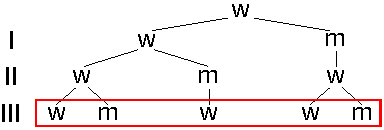
\includegraphics[scale=.75]{Layout.pdf}
	\caption{Aufteilung des Seitenlayouts mit viel Platz f\"{u}r Eure Randnotizen.}
	\label{fig:Seitenlayout}
\end{figure}


% Inhaltsverzeichnis
\tableofcontents
\newpage

\restoregeometry % nutze ab jetzt Notizenrand rechts 5.8.24 J.Hlawatsch

% Einleitung
\chapter{Denkanstöße}\label{Denk}

\begin{itemize}
\item
Warum sollen Menschen (Sch\"{u}lerInnen) Physik erlernen?
\item
Kann man \say{Physik unterrichten} lernen?
\item
K\"{o}nnen Jungen Physik besser verstehen bzw.\ lernen?
\item
Warum sollen im Physikunterricht Experimente durchgef\"{u}hrt werden?
\item
Warum ist Physik das --- mit Abstand --- unbeliebteste Schulfach?
\item
Ist Physikdidaktik eine Wissenschaft?
\item
Warum geht von gro{\ss}en Denkleistungen gerade der Physik eine fast unvergleichliche Faszination aus?
\item
Kann man Physik nur mit Hilfe von Mathematik verstehen?
\item
Ist die Wissenschaft Physik Fluch oder Segen f\"{u}r die Menschheit?
\item
Ist ein Lehrplan f\"{u}r das Unterrichten notwendig?
\item
Sind angesichts von ComputerBeamern noch andere Medien sinnvoll?
\end{itemize}


%\begin{ziele}
%	Hier stehen Ziele	
%\end{ziele}

\begin{uea}
	Beantworten Sie diese Fragen für sich und diskutieren Sie Ihre Gedanken mit Ihrem Nachbarn!
\end{uea}

\newpage

%---------------------------------------------------------------------------------------------------------------------------------

\chapter{Begr\"{u}ndung von Physik in der Schule}\label{Begruendung}

Wie kann Physikunterricht gerechtfertigt ( = legitimiert) werden? \\
Ist es sinnvoll, Physik in der Schule zu unterrichten?

Unter welchen Gesichtspunkten ist diese Frage zu beantworten?
\begin{itemize}
	\item Aus der Sicht des Kindes?
	\item Aus der Sicht der Erziehenden?
	\item Aus der Sicht der Gesellschaft?
	\item Aus der Sicht der Wirtschaft?
\end{itemize}

\begin{enumerate}
	\item Kulturelle Identit\"{a}t

\begin{enumerate}

\item Lange Tradition einer Kultur in Europa, in
Deutschland.

\item Spezifisch naturwissenschaftliche Sichtweise:
\begin{itemize}
\item Naturwissenschaftliche Methode (Falsifikation von Hypothesen).
\item Empirik (Experiment),
\item Mathematisierung,
\item Rationales Argumentieren,
\item Exaktheit,
\end{itemize}

\item Entmythologisierung:
\begin{itemize}
\item ,,Die heilende Strahlkraft der Steine''
\item Astronomie und Astrologie,
\item Die teuflischen Handy-Strahlen.
\end{itemize}

\item Verantwortung f\"{u}r die Welt:
\begin{itemize}
\item Gestaltung der technischen Zivilisation
\item Umwelterziehung:
\begin{itemize}
\item Kann ich anstelle einer Haushalts(Trocken-)Batterie auch ein
Netzger\"{a}t verwenden?
\end{itemize}

\end{itemize}


\item Attribuierungen von Physik:
\begin{itemize}
\item Physik ist nicht nur die Technik-Hybris: Atombomben,
Kraftwerke, Anonyme Apparate-Medizin,
\item
Ehrfurcht vor den Theorien der theoretisch-abstrakten Physik.
\end{itemize}

\end{enumerate}

\item Lebensbew\"{a}ltigung

\begin{enumerate}

\item Handwerklich-technische Fertigkeiten, Berufsbildung
\item Genaues Beobachten.

\begin{itemize}
\item In welcher Reihenfolge treten (welche) Farben im Regenbogen auf?
In welcher Richtung ist der Bogen zu sehen?
\end{itemize}


\item Sprachliche Beschreibung:
\begin{itemize}
\item Stimmige Ausdrucksweisen: Der Strom flie{\ss}t, es liegt ein Spannung an,
\item Bereicherung des Wortschatzes: El.\ Spannung, Druck, Temperatur, Verdampfen, Verdunsten,\dots.
\item Vertrautheit mit Einheiten.
\end{itemize}

\item Sicherheitsbewusstsein:
\begin{itemize}
\item Der F\"{o}hn in der Badewanne,
\item Der Fotoapparat im Schwimmbad,
\item Der Stuhl an der Wand,
\end{itemize}

\end{enumerate}

\item
Im Hinblick auf die Schule: Physik als ,,Methode''

\begin{itemize}
\item Farbe im Unterricht
\item Spielerische Elemente,
\item Handlungsorientierung,
\item Soziale Lernziele: Gruppenexperiment,
\item M\"{o}glichkeit zum Fach\"{u}bergriff:
\begin{itemize}
\item Mathematik: Gr\"{o}{\ss}enrechnen,
\item Verkehrserziehung: Geschwindigkeit, Kr\"{a}fte, Fliehkr\"{a}fte, Bremswege.
\end{itemize}

\end{itemize}

\item Weitere Gesichtspunkte:
\begin{itemize}
\item \"{A}sthetik,
\item M\"{a}dchen und Physik
\item Entwicklung
\end{itemize}

\end{enumerate}


% Erstes Kapitel
\section{Mechanik}
\subsection{Kinematik}
Die Kinematik beschreibt die Bewegung von Punkten und Körpern ohne Berücksichtigung der Kräfte, die diese Bewegungen verursachen.

\subsubsection{Beispiel für eine Formel}
Die Gleichung für die Geschwindigkeit \(v\) in Abhängigkeit von der Zeit \(t\) ist:
\begin{equation}
	E=mc^2
\end{equation}
\begin{equation}
    v(t) = \frac{ds(t)}{dt} \label{franz}
\end{equation}
wobei \(s(t)\) die zurückgelegte Strecke ist. Nach \cref{franz} bla

% Zweites Kapitel
\section{Thermodynamik}
\subsection{Erster Hauptsatz}
Der erste Hauptsatz der Thermodynamik besagt, dass die Energie in einem abgeschlossenen System erhalten bleibt.

\subsubsection{Beispiel für eine Gleichung}
Die Änderung der inneren Energie \( \Delta U \) ist gegeben durch:
\begin{equation}
    \Delta U = Q - W
\end{equation}
wobei \( Q \) die zugeführte Wärme und \( W \) die geleistete Arbeit ist.

% Weitere Kapitel...

% Literaturverzeichnis
\newpage
\begin{thebibliography}{9}
\bibitem{Beispiel1}
Autor, Titel, Verlag, Jahr.

\bibitem{Beispiel2}
Autor, Titel, Verlag, Jahr.
\end{thebibliography}

\end{document}